\subsection{ResNet50}

\paragraph{Evaluación Cuantitativa de ResNet50:}

\subparagraph{Fase Base (30 épocas fijas):}
El modelo ResNet50 fue entrenado durante 30 épocas fijas con una tasa de aprendizaje de $1\times10^{-4}$. Las métricas obtenidas sobre el conjunto de prueba aislado se presentan en la Tabla~\ref{tab:resnet_base_metrics}. La arquitectura residual, que cuenta con 23.51~M de parámetros, alcanzó un accuracy de 99.31\%, un F1-Score de 99.42\% y un AUC-ROC de 0.9995. Estos resultados demuestran una elevada capacidad discriminativa inicial gracias a las conexiones residuales que facilitan el flujo de gradiente a través de las capas profundas.

\begin{table}[H]
\centering
\caption{Métricas de evaluación de ResNet50 en la fase base.}
\label{tab:resnet_base_metrics}
\begin{tabular}{lc}
\hline
Métrica & Valor \\
\hline
Accuracy  & 99.31\% \\
Balanced Accuracy & 99.31\% \\
Precisión & 99.51\% \\
Recall (Sensibilidad) & 99.32\% \\
Especificidad & 99.30\% \\
F1-Score & 99.42\% \\
MCC & 0.9858 \\
AUC-ROC & 0.9995 \\
\hline
\end{tabular}
\end{table}

Durante la fase base, la pérdida de entrenamiento disminuyó progresivamente hasta alcanzar valores cercanos a cero al término de las 30 épocas. La pérdida de validación mostró una estabilización temprana alrededor de la época~8 con un valor de 0.0185, experimentando ligeras fluctuaciones en las épocas finales debido a la ausencia de regularización dinámica y la tasa de aprendizaje constante. A pesar de estas variaciones sintomáticas de una tasa fija, el modelo mantuvo un rendimiento estable sin caer en un sobreajuste severo.

\begin{figure}[H]
\centering
\begin{minipage}{0.45\textwidth}
    \centering
    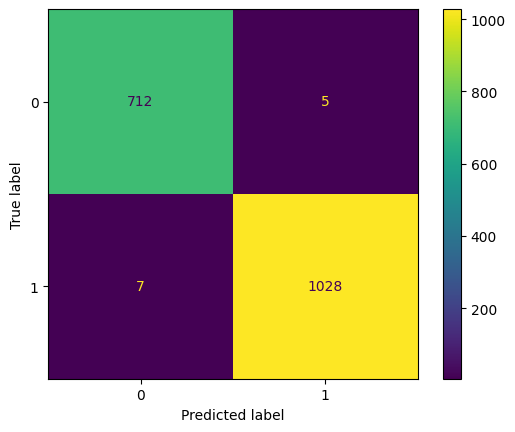
\includegraphics[width=\textwidth]{../BrainTumor/results/resnet50/base/confusion_matrix.png}
    \caption{Matriz de confusión de ResNet50 en la fase base.}
    \label{fig:resnet_base_cm}
\end{minipage}
\hfill
\begin{minipage}{0.45\textwidth}
    \centering
    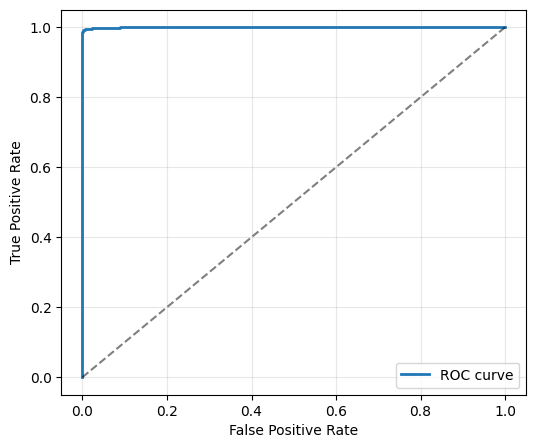
\includegraphics[width=\textwidth]{../BrainTumor/results/resnet50/base/roc_curve.png}
    \caption{Curva ROC de ResNet50 en la fase base.}
    \label{fig:resnet_base_roc}
\end{minipage}
\end{figure}

\subparagraph{Fase Optimizada (Early Stopping y optimización adaptativa):}
En la fase optimizada se incorporaron data augmentation, precisión mixta automática (AMP), regularización por weight decay y el programador ReduceLROnPlateau. El entrenamiento convergió de manera eficiente, deteniéndose mediante early stopping tras registrar la mejor pérdida de validación. La tasa de aprendizaje adaptativa y las técnicas de regularización permitieron que las métricas finales en el conjunto de prueba alcanzaran valores superiores, como se detalla en la Tabla~\ref{tab:resnet_opt_metrics}.

\begin{table}[H]
\centering
\caption{Métricas de evaluación de ResNet50 en la fase optimizada.}
\label{tab:resnet_opt_metrics}
\begin{tabular}{lc}
\hline
Métrica & Valor \\
\hline
Accuracy  & 99.54\% \\
Balanced Accuracy & 99.57\% \\
Precisión & 99.81\% \\
Recall (Sensibilidad) & 99.42\% \\
Especificidad & 99.72\% \\
F1-Score & 99.61\% \\
MCC & 0.9906 \\
AUC-ROC & 0.9998 \\
\hline
\end{tabular}
\end{table}

La optimización redujo los falsos positivos a solo 2 muestras y los falsos negativos a 6 muestras sobre el total de 1752 imágenes de prueba. La combinación de AMP y data augmentation redujo significativamente el consumo de recursos computacionales, registrando un tiempo de inferencia promedio de 108.42~ms por batch. Las mejoras observadas confirman que la regularización adaptativa optimiza el espacio de parámetros de ResNet50, aumentando tanto la sensibilidad diagnóstica como la especificidad.

\begin{figure}[H]
\centering
\begin{minipage}{0.45\textwidth}
    \centering
    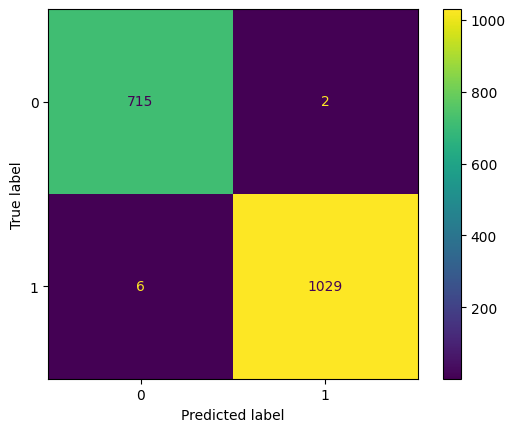
\includegraphics[width=\textwidth]{../BrainTumor/results/resnet50/optimized/confusion_matrix.png}
    \caption{Matriz de confusión de ResNet50 optimizado.}
    \label{fig:resnet_opt_cm}
\end{minipage}
\hfill
\begin{minipage}{0.45\textwidth}
    \centering
    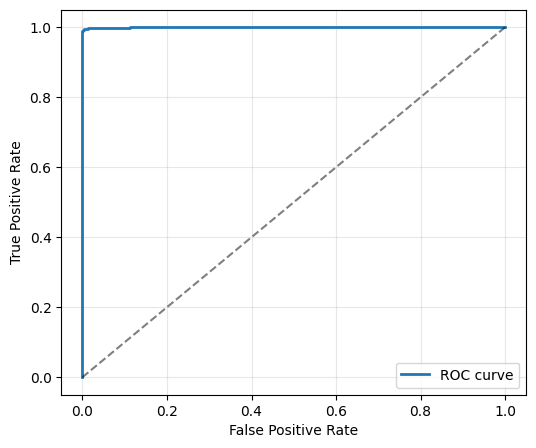
\includegraphics[width=\textwidth]{../BrainTumor/results/resnet50/optimized/roc_curve.png}
    \caption{Curva ROC de ResNet50 optimizado.}
    \label{fig:resnet_opt_roc}
\end{minipage}
\end{figure}

\paragraph{Matriz de Confusión y Curvas de Aprendizaje:}

El análisis comparativo de las curvas de aprendizaje evidencia que las conexiones residuales de ResNet50 facilitan una convergencia rápida y estable. En la fase base, la curva de train\_loss descendió de manera continua mientras que val\_loss alcanzó un mínimo estable, aunque con oscilaciones menores en las épocas superiores causadas por la falta de decaimiento en la tasa de aprendizaje. En la fase optimizada, el programador ReduceLROnPlateau y el early stopping previnieron la sobreestimación de pesos, manteniendo la pérdida de validación en niveles óptimos antes de la detención del entrenamiento.

Las matrices de confusión (Figuras~\ref{fig:resnet_base_cm} y \ref{fig:resnet_opt_cm}) muestran una drástica reducción de errores en la fase optimizada. En la fase base se contabilizaron 5 falsos positivos y 7 falsos negativos (12 errores totales), mientras que en la fase optimizada estos errores descendieron a 2 falsos positivos y 6 falsos negativos (8 errores totales). Esta reducción del 33.3\% en los errores globales de clasificación se refleja directamente en el incremento del F1-Score de 99.42\% a 99.61\% y del MCC de 0.9858 a 0.9906. La curva ROC (Figura~\ref{fig:resnet_opt_roc}) alcanza un AUC-ROC de 0.9998, demostrando una capacidad de separación casi perfecta entre la presencia y ausencia de tumor cerebral.